% Graphic for TeX using PGF
% Title: /home/braulio/Drive/Facultad/Tercero/Segundo_Cuatrimestre/IC/Practicas/PFinal/memoria/modulos.tex
% Creator: Dia v0.97.3
% CreationDate: Sat Jun 25 21:58:06 2016
% For: braulio
% \usepackage{tikz}
% The following commands are not supported in PSTricks at present
% We define them conditionally, so when they are implemented,
% this pgf file will use them.
\ifx\du\undefined
  \newlength{\du}
\fi
\setlength{\du}{15\unitlength}
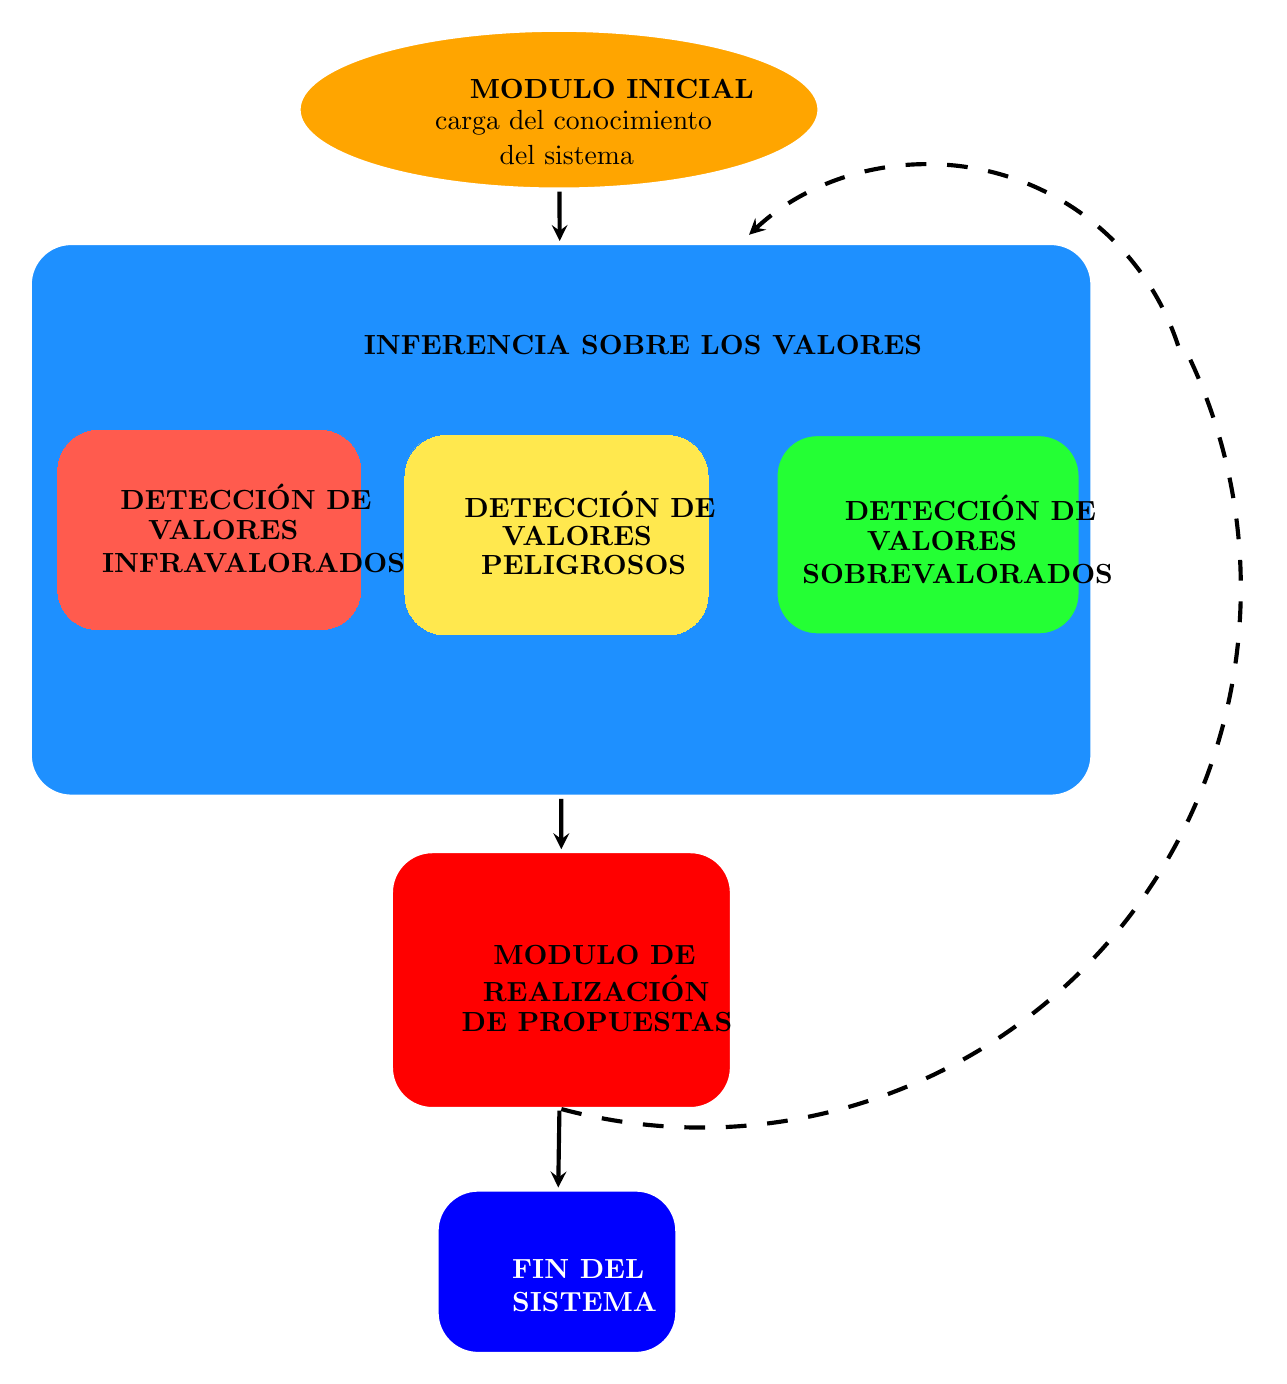
\begin{tikzpicture}
\pgftransformxscale{1.000000}
\pgftransformyscale{-1.000000}
\definecolor{dialinecolor}{rgb}{0.000000, 0.000000, 0.000000}
\pgfsetstrokecolor{dialinecolor}
\definecolor{dialinecolor}{rgb}{1.000000, 1.000000, 1.000000}
\pgfsetfillcolor{dialinecolor}
\definecolor{dialinecolor}{rgb}{1.000000, 0.647059, 0.000000}
\pgfsetfillcolor{dialinecolor}
\pgfpathellipse{\pgfpoint{23.400000\du}{-0.162500\du}}{\pgfpoint{6.275000\du}{0\du}}{\pgfpoint{0\du}{1.925000\du}}
\pgfusepath{fill}
\pgfsetlinewidth{0.100000\du}
\pgfsetdash{}{0pt}
\pgfsetdash{}{0pt}
\definecolor{dialinecolor}{rgb}{1.000000, 1.000000, 1.000000}
\pgfsetstrokecolor{dialinecolor}
\pgfpathellipse{\pgfpoint{23.400000\du}{-0.162500\du}}{\pgfpoint{6.275000\du}{0\du}}{\pgfpoint{0\du}{1.925000\du}}
\pgfusepath{stroke}
\pgfsetlinewidth{0.100000\du}
\pgfsetdash{}{0pt}
\pgfsetdash{}{0pt}
\pgfsetroundjoin
{\pgfsetcornersarced{\pgfpoint{1.000000\du}{1.000000\du}}\definecolor{dialinecolor}{rgb}{0.117647, 0.564706, 1.000000}
\pgfsetfillcolor{dialinecolor}
\fill (10.650000\du,3.050000\du)--(10.650000\du,16.387500\du)--(36.250000\du,16.387500\du)--(36.250000\du,3.050000\du)--cycle;
}{\pgfsetcornersarced{\pgfpoint{1.000000\du}{1.000000\du}}\definecolor{dialinecolor}{rgb}{1.000000, 1.000000, 1.000000}
\pgfsetstrokecolor{dialinecolor}
\draw (10.650000\du,3.050000\du)--(10.650000\du,16.387500\du)--(36.250000\du,16.387500\du)--(36.250000\du,3.050000\du)--cycle;
}\pgfsetlinewidth{0.100000\du}
\pgfsetdash{}{0pt}
\pgfsetdash{}{0pt}
\pgfsetbuttcap
{
\definecolor{dialinecolor}{rgb}{0.000000, 0.000000, 0.000000}
\pgfsetfillcolor{dialinecolor}
% was here!!!
\pgfsetarrowsend{stealth}
\definecolor{dialinecolor}{rgb}{0.000000, 0.000000, 0.000000}
\pgfsetstrokecolor{dialinecolor}
\draw (23.409991\du,1.812061\du)--(23.416002\du,2.999874\du);
}
% setfont left to latex
\definecolor{dialinecolor}{rgb}{0.000000, 0.000000, 0.000000}
\pgfsetstrokecolor{dialinecolor}
\node[anchor=west] at (19.700000\du,-0.662500\du){\textbf{~~~~~MODULO INICIAL}};
% setfont left to latex
\definecolor{dialinecolor}{rgb}{0.000000, 0.000000, 0.000000}
\pgfsetstrokecolor{dialinecolor}
\node[anchor=west] at (19.700000\du,0.137500\du){~~carga del conocimiento};
% setfont left to latex
\definecolor{dialinecolor}{rgb}{0.000000, 0.000000, 0.000000}
\pgfsetstrokecolor{dialinecolor}
\node[anchor=west] at (19.700000\du,0.937500\du){~~~~~~~~~del sistema};
% setfont left to latex
\definecolor{dialinecolor}{rgb}{0.000000, 0.000000, 0.000000}
\pgfsetstrokecolor{dialinecolor}
\node[anchor=west] at (18.425000\du,5.512500\du){\textbf{INFERENCIA SOBRE LOS VALORES}};
\pgfsetlinewidth{0.000000\du}
\pgfsetdash{}{0pt}
\pgfsetdash{}{0pt}
\pgfsetroundjoin
{\pgfsetcornersarced{\pgfpoint{1.000000\du}{1.000000\du}}\definecolor{dialinecolor}{rgb}{1.000000, 0.356863, 0.305882}
\pgfsetfillcolor{dialinecolor}
\fill (11.300000\du,7.537500\du)--(11.300000\du,12.387500\du)--(18.650000\du,12.387500\du)--(18.650000\du,7.537500\du)--cycle;
}{\pgfsetcornersarced{\pgfpoint{1.000000\du}{1.000000\du}}\definecolor{dialinecolor}{rgb}{0.117647, 0.564706, 1.000000}
\pgfsetstrokecolor{dialinecolor}
\draw (11.300000\du,7.537500\du)--(11.300000\du,12.387500\du)--(18.650000\du,12.387500\du)--(18.650000\du,7.537500\du)--cycle;
}% setfont left to latex
\definecolor{dialinecolor}{rgb}{0.000000, 0.000000, 0.000000}
\pgfsetstrokecolor{dialinecolor}
\node[anchor=west] at (11.725000\du,9.162500\du){~~~~\textbf{DETECCIÓN DE }};
% setfont left to latex
\definecolor{dialinecolor}{rgb}{0.000000, 0.000000, 0.000000}
\pgfsetstrokecolor{dialinecolor}
\node[anchor=west] at (11.725000\du,9.962500\du){~~~~~~~\textbf{VALORES}};
% setfont left to latex
\definecolor{dialinecolor}{rgb}{0.000000, 0.000000, 0.000000}
\pgfsetstrokecolor{dialinecolor}
\node[anchor=west] at (11.725000\du,10.762500\du){~~\textbf{INFRAVALORADOS}};
\pgfsetlinewidth{0.100000\du}
\pgfsetdash{}{0pt}
\pgfsetdash{}{0pt}
\pgfsetroundjoin
{\pgfsetcornersarced{\pgfpoint{1.000000\du}{1.000000\du}}\definecolor{dialinecolor}{rgb}{0.141176, 1.000000, 0.203922}
\pgfsetfillcolor{dialinecolor}
\fill (28.615000\du,7.652500\du)--(28.615000\du,12.502500\du)--(35.965000\du,12.502500\du)--(35.965000\du,7.652500\du)--cycle;
}{\pgfsetcornersarced{\pgfpoint{1.000000\du}{1.000000\du}}\definecolor{dialinecolor}{rgb}{0.117647, 0.564706, 1.000000}
\pgfsetstrokecolor{dialinecolor}
\draw (28.615000\du,7.652500\du)--(28.615000\du,12.502500\du)--(35.965000\du,12.502500\du)--(35.965000\du,7.652500\du)--cycle;
}% setfont left to latex
\definecolor{dialinecolor}{rgb}{0.000000, 0.000000, 0.000000}
\pgfsetstrokecolor{dialinecolor}
\node[anchor=west] at (28.990000\du,9.427500\du){\textbf{~~~~DETECCIÓN DE }};
% setfont left to latex
\definecolor{dialinecolor}{rgb}{0.000000, 0.000000, 0.000000}
\pgfsetstrokecolor{dialinecolor}
\node[anchor=west] at (28.990000\du,10.227500\du){~~~~~~~\textbf{VALORES} };
% setfont left to latex
\definecolor{dialinecolor}{rgb}{0.000000, 0.000000, 0.000000}
\pgfsetstrokecolor{dialinecolor}
\node[anchor=west] at (28.990000\du,11.027500\du){ \textbf{SOBREVALORADOS}};
\pgfsetlinewidth{0.100000\du}
\pgfsetdash{}{0pt}
\pgfsetdash{}{0pt}
\pgfsetroundjoin
{\pgfsetcornersarced{\pgfpoint{1.000000\du}{1.000000\du}}\definecolor{dialinecolor}{rgb}{1.000000, 0.000000, 0.000000}
\pgfsetfillcolor{dialinecolor}
\fill (19.350000\du,17.700000\du)--(19.350000\du,23.912500\du)--(27.565000\du,23.912500\du)--(27.565000\du,17.700000\du)--cycle;
}{\pgfsetcornersarced{\pgfpoint{1.000000\du}{1.000000\du}}\definecolor{dialinecolor}{rgb}{1.000000, 1.000000, 1.000000}
\pgfsetstrokecolor{dialinecolor}
\draw (19.350000\du,17.700000\du)--(19.350000\du,23.912500\du)--(27.565000\du,23.912500\du)--(27.565000\du,17.700000\du)--cycle;
}\pgfsetlinewidth{0.100000\du}
\pgfsetdash{}{0pt}
\pgfsetdash{}{0pt}
\pgfsetbuttcap
{
\definecolor{dialinecolor}{rgb}{0.000000, 0.000000, 0.000000}
\pgfsetfillcolor{dialinecolor}
% was here!!!
\pgfsetarrowsend{stealth}
\definecolor{dialinecolor}{rgb}{0.000000, 0.000000, 0.000000}
\pgfsetstrokecolor{dialinecolor}
\draw (23.454545\du,16.437637\du)--(23.455367\du,17.652701\du);
}
% setfont left to latex
\definecolor{dialinecolor}{rgb}{0.000000, 0.000000, 0.000000}
\pgfsetstrokecolor{dialinecolor}
\node[anchor=west] at (20.782500\du,20.213800\du){\textbf{~~~MODULO DE }};
% setfont left to latex
\definecolor{dialinecolor}{rgb}{0.000000, 0.000000, 0.000000}
\pgfsetstrokecolor{dialinecolor}
\node[anchor=west] at (20.782500\du,21.013800\du){\textbf{~~REALIZACIÓN }};
% setfont left to latex
\definecolor{dialinecolor}{rgb}{0.000000, 0.000000, 0.000000}
\pgfsetstrokecolor{dialinecolor}
\node[anchor=west] at (20.782500\du,21.813800\du){\textbf{DE PROPUESTAS}};
\pgfsetlinewidth{0.100000\du}
\pgfsetdash{{1.000000\du}{1.000000\du}}{0\du}
\pgfsetdash{{0.500000\du}{0.500000\du}}{0\du}
\pgfsetbuttcap
{
\definecolor{dialinecolor}{rgb}{0.000000, 0.000000, 0.000000}
\pgfsetfillcolor{dialinecolor}
% was here!!!
\definecolor{dialinecolor}{rgb}{0.000000, 0.000000, 0.000000}
\pgfsetstrokecolor{dialinecolor}
\pgfpathmoveto{\pgfpoint{23.456557\du}{23.912261\du}}
\pgfpatharc{105}{-27}{13.002537\du and 13.002537\du}
\pgfusepath{stroke}
}
\pgfsetlinewidth{0.100000\du}
\pgfsetdash{{0.500000\du}{0.500000\du}}{0\du}
\pgfsetdash{{0.500000\du}{0.500000\du}}{0\du}
\pgfsetbuttcap
{
\definecolor{dialinecolor}{rgb}{0.000000, 0.000000, 0.000000}
\pgfsetfillcolor{dialinecolor}
% was here!!!
\pgfsetarrowsend{stealth}
\definecolor{dialinecolor}{rgb}{0.000000, 0.000000, 0.000000}
\pgfsetstrokecolor{dialinecolor}
\pgfpathmoveto{\pgfpoint{38.314411\du}{5.524513\du}}
\pgfpatharc{342}{227}{6.329669\du and 6.329669\du}
\pgfusepath{stroke}
}
\pgfsetlinewidth{0.100000\du}
\pgfsetdash{}{0pt}
\pgfsetdash{}{0pt}
\pgfsetroundjoin
{\pgfsetcornersarced{\pgfpoint{1.000000\du}{1.000000\du}}\definecolor{dialinecolor}{rgb}{0.000000, 0.000000, 1.000000}
\pgfsetfillcolor{dialinecolor}
\fill (20.450000\du,25.852500\du)--(20.450000\du,29.812500\du)--(26.250000\du,29.812500\du)--(26.250000\du,25.852500\du)--cycle;
}{\pgfsetcornersarced{\pgfpoint{1.000000\du}{1.000000\du}}\definecolor{dialinecolor}{rgb}{1.000000, 1.000000, 1.000000}
\pgfsetstrokecolor{dialinecolor}
\draw (20.450000\du,25.852500\du)--(20.450000\du,29.812500\du)--(26.250000\du,29.812500\du)--(26.250000\du,25.852500\du)--cycle;
}% setfont left to latex
\definecolor{dialinecolor}{rgb}{1.000000, 1.000000, 1.000000}
\pgfsetstrokecolor{dialinecolor}
\node[anchor=west] at (22.000000\du,27.762500\du){ \textcolor{white}{\textbf{FIN DEL}}};
% setfont left to latex
\definecolor{dialinecolor}{rgb}{1.000000, 1.000000, 1.000000}
\pgfsetstrokecolor{dialinecolor}
\node[anchor=west] at (22.000000\du,28.562500\du){\textcolor{white}{\textbf{SISTEMA}}};
\pgfsetlinewidth{0.100000\du}
\pgfsetdash{}{0pt}
\pgfsetdash{}{0pt}
\pgfsetbuttcap
{
\definecolor{dialinecolor}{rgb}{0.000000, 0.000000, 0.000000}
\pgfsetfillcolor{dialinecolor}
% was here!!!
\pgfsetarrowsend{stealth}
\definecolor{dialinecolor}{rgb}{0.000000, 0.000000, 0.000000}
\pgfsetstrokecolor{dialinecolor}
\draw (23.409419\du,23.948850\du)--(23.381055\du,25.802761\du);
}
\pgfsetlinewidth{0.000000\du}
\pgfsetdash{}{0pt}
\pgfsetdash{}{0pt}
\pgfsetroundjoin
{\pgfsetcornersarced{\pgfpoint{1.000000\du}{1.000000\du}}\definecolor{dialinecolor}{rgb}{1.000000, 0.909804, 0.305882}
\pgfsetfillcolor{dialinecolor}
\fill (19.665000\du,7.665000\du)--(19.665000\du,12.515000\du)--(27.015000\du,12.515000\du)--(27.015000\du,7.665000\du)--cycle;
}{\pgfsetcornersarced{\pgfpoint{1.000000\du}{1.000000\du}}\definecolor{dialinecolor}{rgb}{0.117647, 0.564706, 1.000000}
\pgfsetstrokecolor{dialinecolor}
\draw (19.665000\du,7.665000\du)--(19.665000\du,12.515000\du)--(27.015000\du,12.515000\du)--(27.015000\du,7.665000\du)--cycle;
}% setfont left to latex
\definecolor{dialinecolor}{rgb}{0.000000, 0.000000, 0.000000}
\pgfsetstrokecolor{dialinecolor}
\node[anchor=west] at (20.900000\du,9.350000\du){\textbf{DETECCIÓN DE}};
% setfont left to latex
\definecolor{dialinecolor}{rgb}{0.000000, 0.000000, 0.000000}
\pgfsetstrokecolor{dialinecolor}
\node[anchor=west] at (21.800000\du,10.100000\du){\textbf{VALORES}};
% setfont left to latex
\definecolor{dialinecolor}{rgb}{0.000000, 0.000000, 0.000000}
\pgfsetstrokecolor{dialinecolor}
\node[anchor=west] at (21.300000\du,10.800000\du){\textbf{PELIGROSOS}};
\end{tikzpicture}
